

%\usepackage{graphicx}   % for EPS use the graphics package instead


%\begin{figure}
 
%\begin{center}

%   \resizebox{!}{50mm}{\includegraphics[width=1\textwidth]{.png}}
% 	 \caption{\emph{}}
  

%\end{center}    
%\end{figure}



%\subsection{Virtual Window}
\begin{figure}
\begin{center}
  \resizebox{!}{50mm}{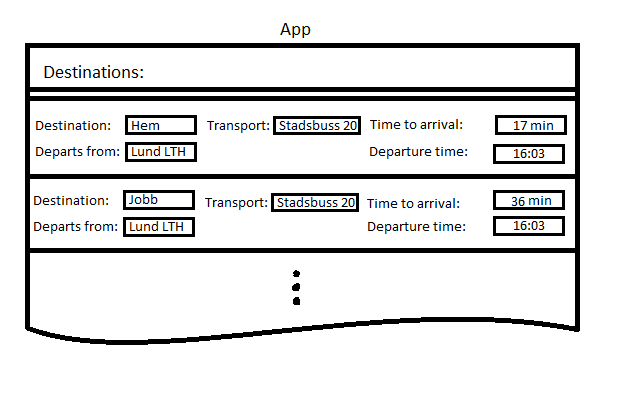
\includegraphics[width=1\textwidth]{Screens/vwApp.png}}
  \caption{\emph{Virtual Window for the Application}} \label{pic:vwApp}
\end{center}    
\end{figure}

%=============================================================================
%       Next picture
%=============================================================================

\begin{figure}
\begin{center}
  \resizebox{!}{50mm}{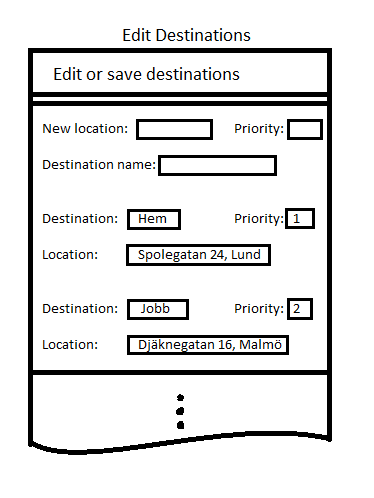
\includegraphics[width=1\textwidth]{Screens/vwEdit.png}}
  \caption{\emph{Virtual Window for editing destinations}} \label{pic:vwEdit}  
\end{center}    
\end{figure}

%=============================================================================
%       Next picture
%=============================================================================

\begin{figure}
\begin{center}
  \resizebox{!}{50mm}{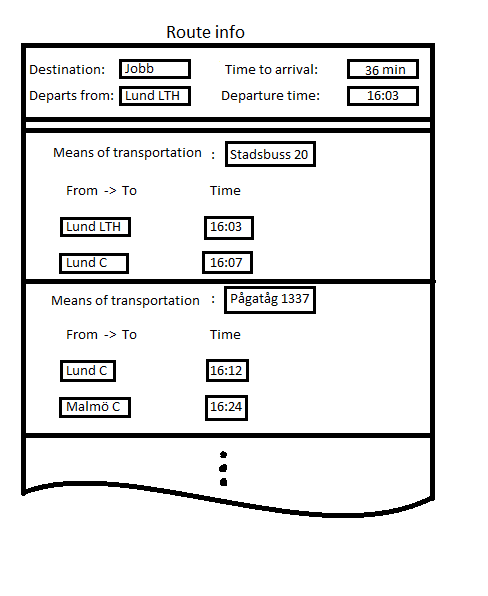
\includegraphics[width=1\textwidth]{Screens/vwRoute.png}}
  \caption{\emph{Virtual Window for the route information}} \label{pic:vwRoute}
\end{center}    
\end{figure}

%=============================================================================
%       Next picture
%=============================================================================

\begin{figure}
\begin{center}
  \resizebox{!}{50mm}{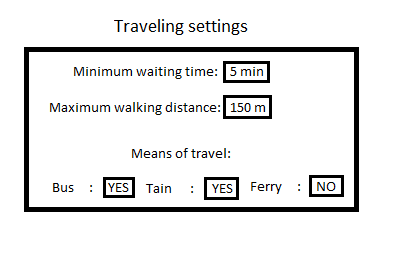
\includegraphics[width=1\textwidth]{Screens/vwSettings.png}}
  \caption{\emph{Virtual Window for the Traveling Settings}} \label{pic:vwSettings}
\end{center}    
\end{figure}

%=============================================================================
%       Next picture
%=============================================================================

\begin{figure}
\begin{center}
  \resizebox{!}{50mm}{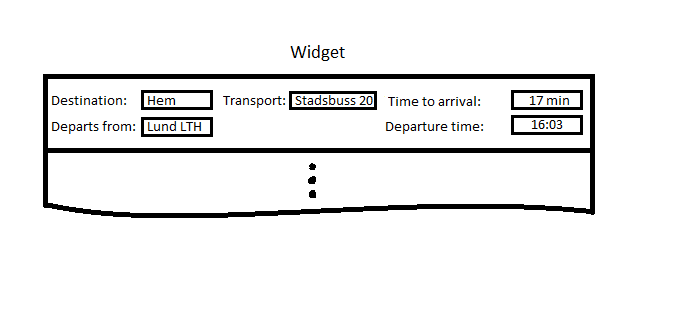
\includegraphics[width=1\textwidth]{Screens/vwWidget.png}}
  \caption{\emph{Virtual Window for the Widget}} \label{pic:vwWidget}
\end{center}    
\end{figure}

%=============================================================================
%       Next picture
%=============================================================================

\begin{figure}
\begin{center}
  \resizebox{!}{50mm}{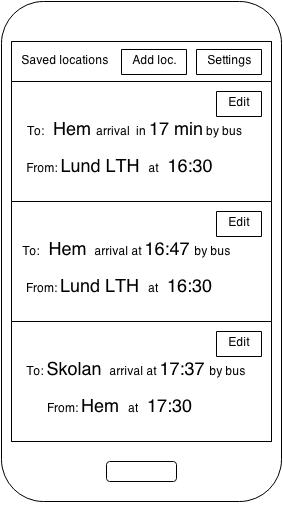
\includegraphics[width=1\textwidth]{Screens/Application.png}}
  \caption{\emph{A view of the Application main window}} \label{pic:Application}
\end{center}    
\end{figure}

%=============================================================================
%       Next picture
%=============================================================================

\begin{figure}
\begin{center}
  \resizebox{!}{50mm}{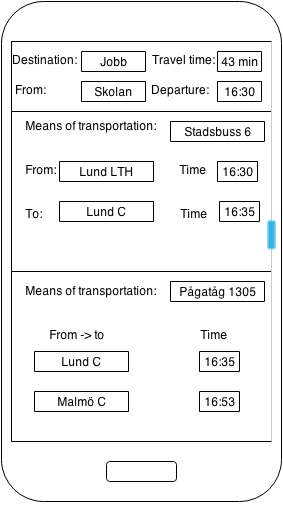
\includegraphics[width=1\textwidth]{Screens/TripInformation.png}}
  \caption{\emph{A view of the detailed information about a trip}} \label{pic:TripInformation}
\end{center}    
\end{figure}

%=============================================================================
%       Next picture
%=============================================================================

\begin{figure}
\begin{center}
  \resizebox{!}{50mm}{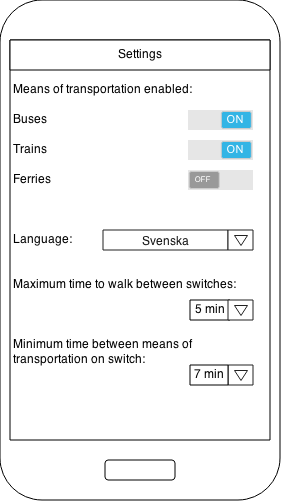
\includegraphics[width=1\textwidth]{Screens/Settings.png}}
  \caption{\emph{A view of the Settings window}} \label{pic:Settings}
\end{center}    
\end{figure}

%=============================================================================
%       Next picture
%=============================================================================

\begin{figure}
\begin{center}
  \resizebox{!}{50mm}{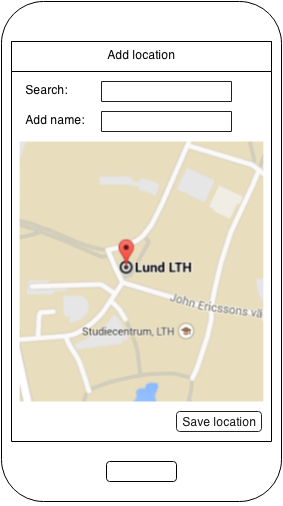
\includegraphics[width=1\textwidth]{Screens/AddDestination.png}}
  \caption{\emph{A view of the window for adding a new destination}} \label{AddDestination}
\end{center}    
\end{figure}

%=============================================================================
%       Next picture
%=============================================================================

\begin{figure}
\begin{center}
  \resizebox{!}{50mm}{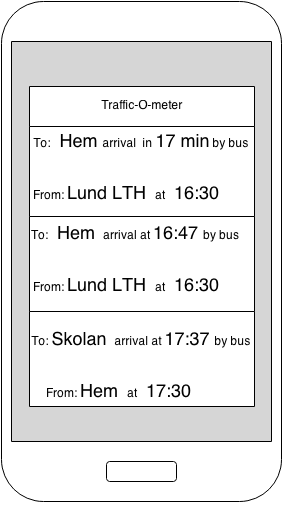
\includegraphics[width=1\textwidth]{Screens/widget.png}}
  \caption{\emph{A view of the Widget}} \label{pic:widget}
\end{center}    
\end{figure}

